\section{Core Pressure, Confinement, and the Mechanical Origin of Mass and Time}

\subsection{Radial Pressure Field and Core Confinement}

In the VAM framework, every knotted vortex structure generates a radial pressure gradient due to its circulating swirl. The pressure field obeys:
\[
P(r) = \frac{1}{2} \rho_{\ae} \left( \frac{\Gamma}{2\pi r} \right)^2 = \frac{\rho_{\ae} \Gamma^2}{8\pi^2 r^2}
\]
To avoid divergence at \( r = 0 \), a finite core radius \( r_c \) is imposed, marking the transition from solid-body swirl to irrotational flow. The pressure at the core boundary reaches a maximum:
\[
P_{\text{max}} = \frac{1}{2} \rho_{\ae} C_e^2 \approx 2.3\,\text{GPa}
\]

This pressure spike corresponds to the maximum internal æther stress the vortex can sustain and constitutes the mechanical origin of rest mass and temporal drag at the swirl center.

\subsection{Mass from Swirl Confinement}
\label{subsec:mass-from-swirl}

VAM replaces symmetry-breaking with swirl mechanics: the inertial mass of a vortex excitation arises from the energy trapped in its core swirl. This is given by:
\[
m_f = \frac{\rho_{\ae} \Gamma^2}{3\pi r_c c^2}
\]
This expression highlights that mass is not fundamental but emergent from:
\begin{itemize}
    \item The circulation strength \( \Gamma \),
    \item The confinement scale \( r_c \),
    \item The æther density \( \rho_{\ae} \),
    \item And the swirl propagation limit \( c \).
\end{itemize}
Unlike the Higgs mechanism, no scalar field is needed—mass is fluid inertia stabilized by swirl-bound curvature over \( T_v \).

\subsection{Smoothed Core Profile}

To ensure physical continuity, the velocity and pressure fields are defined piecewise:
\[
v_\theta(r) =
\begin{cases}
\frac{\Gamma r}{2\pi r_c^2}, & r \leq r_c \\
\frac{\Gamma}{2\pi r}, & r > r_c
\end{cases}
\quad
P(r) =
\begin{cases}
\frac{\rho_{\ae} \Gamma^2 r^2}{8\pi^2 r_c^4}, & r \leq r_c \\
\frac{\rho_{\ae} \Gamma^2}{8\pi^2 r^2}, & r > r_c
\end{cases}
\]

This core smoothing maintains finite energy and avoids singular accelerations during temporal evolution across \( S(t) \).

\subsection{Boundary Layer and Ætheric Equilibrium}

As pressure decays with radial distance, equilibrium with the background æther field is restored near:
\[
R_{\text{eq}} \sim a_0 = \frac{4\pi \varepsilon_0 \hbar^2}{m_e e^2} \approx 5.29 \times 10^{-11} \, \text{m}
\]
This coincidence with the Bohr radius implies that atomic orbital size corresponds to hydrodynamic pressure equilibrium—suggesting that chemical boundaries arise from fluid tension, not probabilistic wavefunctions.

\subsection{Ætheric Time Dilation from Swirl Pressure}

Time dilation in VAM results from internal swirl stress, not relative velocity or spacetime curvature. From Bernoulli pressure–velocity relations, we obtain:
\[
\frac{d\tau}{dt} = \sqrt{1 - \frac{v_\theta^2}{c^2}} \approx 1 - \frac{P(r)}{\rho_{\ae} c^2}
\]
At the core boundary:
\[
\frac{d\tau}{dt} \approx 1 - \left( \frac{C_e}{c} \right)^2 \approx 1 - 6.5 \times 10^{-10}
\]
This demonstrates that proper time \( \tau \) slows in high-pressure swirl zones—linking internal vortex evolution over \( T_v \) to observable clock rates \( d\tau/dt \) in \( \bar{t} \).

\begin{figure}[H]
\centering
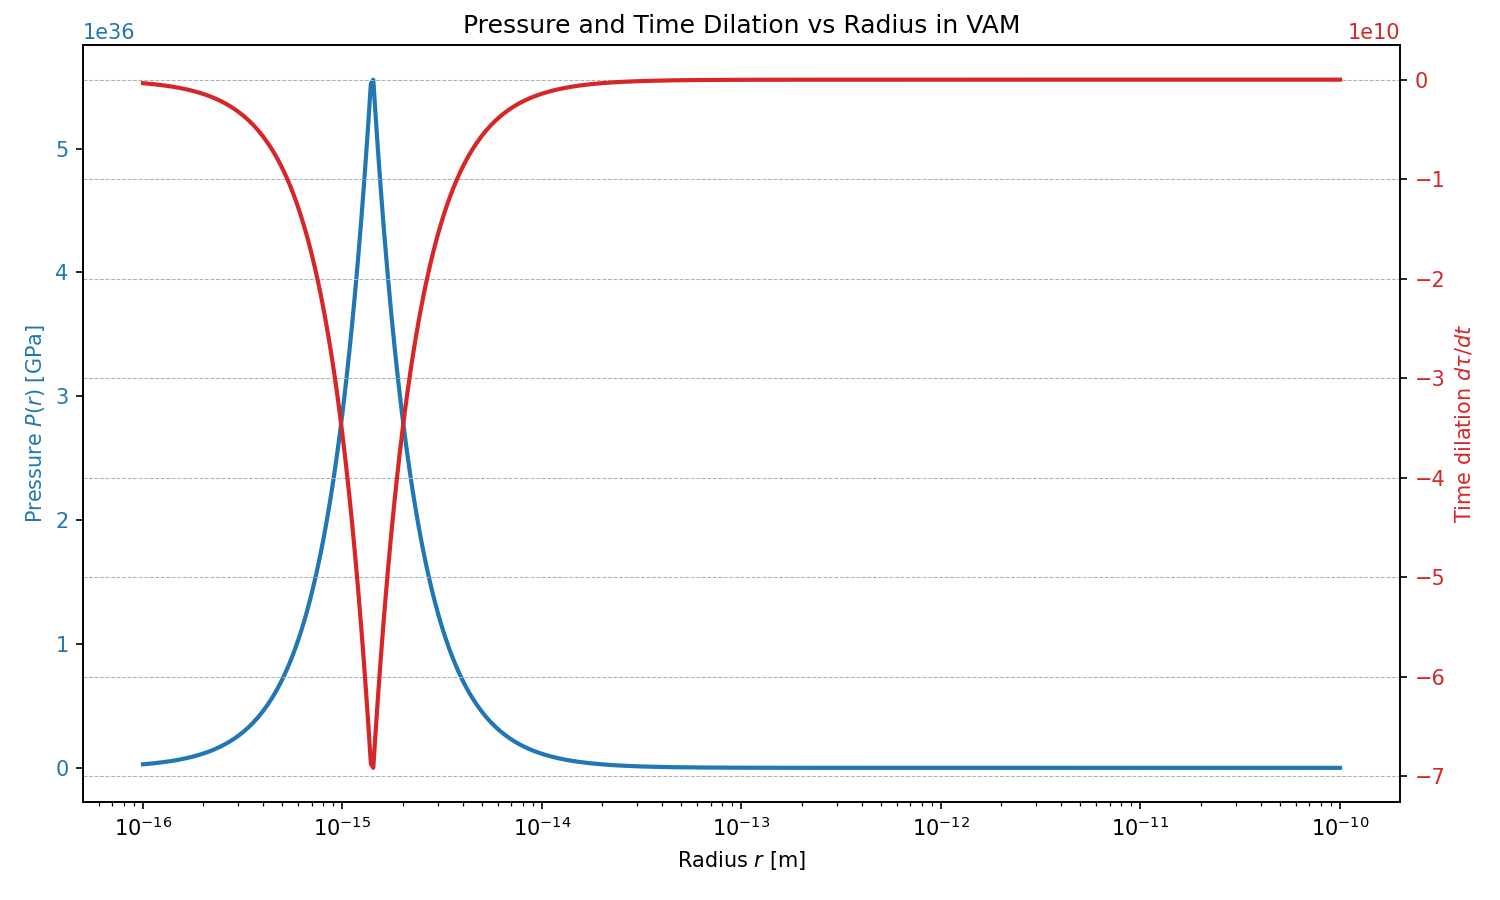
\includegraphics[width=0.85\textwidth]{images/TimeDilationCore}
\caption{
\textbf{Radial profile of swirl-induced pressure and time dilation.} Swirl pressure peaks near \( r_c \sim 10^{-15} \,\mathrm{m} \), inducing a drop in \( d\tau/dt \). The red curve shows clock slowing inside the core due to fluid stress. This effect is fundamental to temporal ontology in VAM, replacing spacetime curvature with rotational æther stress.
}
\label{fig:time_dilation_profile}
\end{figure}

\subsection{Mechanical Ontology Summary}

\begin{table}[H]
\centering
\small
\renewcommand{\arraystretch}{1.4}
\begin{tabular}{|l|l|l|}
\hline
\textbf{Feature} & \textbf{VAM Description} & \textbf{Standard Model Analogy} \\
\hline
Core Pressure & Swirl-induced confinement & QCD bag model \\
Mass & Vortex swirl inertia & Higgs field amplitude \\
Boundary Shell \( R_{\text{eq}} \) & Pressure equalization radius & Bohr radius (electron cloud) \\
Time Dilation & Ætheric swirl stress & General relativistic redshift \\
Inertia & Topological swirl resistance & Unexplained (postulated) \\
\hline
\end{tabular}
\caption{Mapping of mass and time generation in VAM vs. the Standard Model.}
\end{table}

\subsection*{Final Insight}

The 2.3–2.5 GPa core pressure stabilizes vortex-bound structures and causes local slowdown of swirl clocks \( S(t) \). This simultaneously generates:
\begin{itemize}
  \item Mass (via confined kinetic energy),
  \item Time dilation (via helicity drag),
  \item Spatial boundaries (via pressure equilibrium).
\end{itemize}
Together, these effects offer a purely mechanical basis for mass, inertia, and proper time.

\section{Knotted Vortex Molecules and Swirl-Mediated Binding}

Recent developments in gravitating multi-body systems show that field-mediated forces can produce \emph{molecular-like} bound states without direct contact. In VAM, we extend this to topological fluid systems: knots can form bound \textit{vortex molecules} by exchanging swirl field modes across the background æther.

\subsubsection*{Swirl Coupling Potential Between Knots}

Let \( |K_1\rangle \), \( |K_2\rangle \) be two knots characterized by \( T_i, C_i, Lk_i \). The inter-vortex potential is modeled as:
\[
V_{\text{int}}(r, \Delta T, \Delta C) \sim -\frac{\Gamma^2}{r^n} \cos(\omega_{\text{res}} t)
\]
This arises from resonant phase coupling between \( S(t) \)-oscillations of the knots, modulated by helicity configuration and circulation gradient. The resonance frequency \( \omega_{\text{res}} \) depends on relative twist and chirality.

\subsubsection*{Resonance Quantization}

Swirl-mediated binding becomes energetically favorable when:
\[
\omega_{\text{res}} = \frac{2\pi n}{L_{\text{eff}}}, \quad n \in \mathbb{Z}
\]
These are the standing wave modes in the inter-knot swirl tube of length \( L_{\text{eff}} \). This condition stabilizes vortex molecules and defines their mass–frequency spectrum.

\subsubsection*{Topological Quantum Numbers}

Each vortex molecule possesses:
\begin{itemize}
  \item Link number: \( Q = \text{Link}(K_1, K_2) \)
  \item Composite twist: \( T_{\text{tot}} = T_1 + T_2 + T_{\text{exchange}} \)
  \item Chirality factor: \( C_{\text{eff}} = C_1 \cdot C_2 \)
\end{itemize}

These invariants determine the coupling strength, the mode spectrum, and the long-term temporal behavior of the bound system across \( T_v \).

\subsubsection*{Topological Stability and Confinement}

Like color confinement in QCD, some vortex knots (e.g. with \( Q \neq 0 \)) are only stable when part of a bound molecule. For example:
\begin{itemize}
  \item Triskelion triplets model baryons,
  \item Vortex dipoles model mesons,
  \item Higher linkings model exotic hadrons.
\end{itemize}

These are stabilized by swirl-mediated coherence over \( \mathcal{N} \), not by field-theoretic vacuum expectation values.

